\documentclass[12pt]{beamer}

\usetheme{metropolis}
\usepackage{appendixnumberbeamer}

\usepackage{booktabs}
\usepackage[scale=2]{ccicons}

\usepackage{pgfplots}
\usepgfplotslibrary{dateplot}

\usepackage{xspace}
\newcommand{\themename}{\textbf{\textsc{metropolis}}\xspace}



\title{Introduction to CTFs}
\subtitle{What are CTFs and how to get started}
\date{\today}
\author{LosFuzzys}
% \institute{TU}
% \titlegraphic{\hfill\includegraphics[height=1.5cm]{logo.pdf}}

\begin{document}

\maketitle

% \begin{frame}{Table of contents}
%   \setbeamertemplate{section in toc}[sections numbered]
%   \tableofcontents[hideallsubsections]
% \end{frame}

\section{Introduction}

\begin{frame}{\$whoarewe}
    \hspace*{-1cm}%
    \begin{tabular}{cl}
        \begin{tabular}{l}
            \parbox{0.6\linewidth}{%  change the parbox width as appropiate
                \begin{itemize}
                    \item ~15 active Member
                    \item Meet every Wednesday 18:15
                    \item Regular compeeting in security copmetitions
                    \item Host CTFs, trainings and workshops
                \end{itemize}
            }
        \end{tabular}  &
        \begin{tabular}{c}
            \begin{figure}
                \includegraphics[width=0.45\linewidth,]{images/events/Beginnertrainings2022.jpg}
            \end{figure} \\
            \begin{figure}
                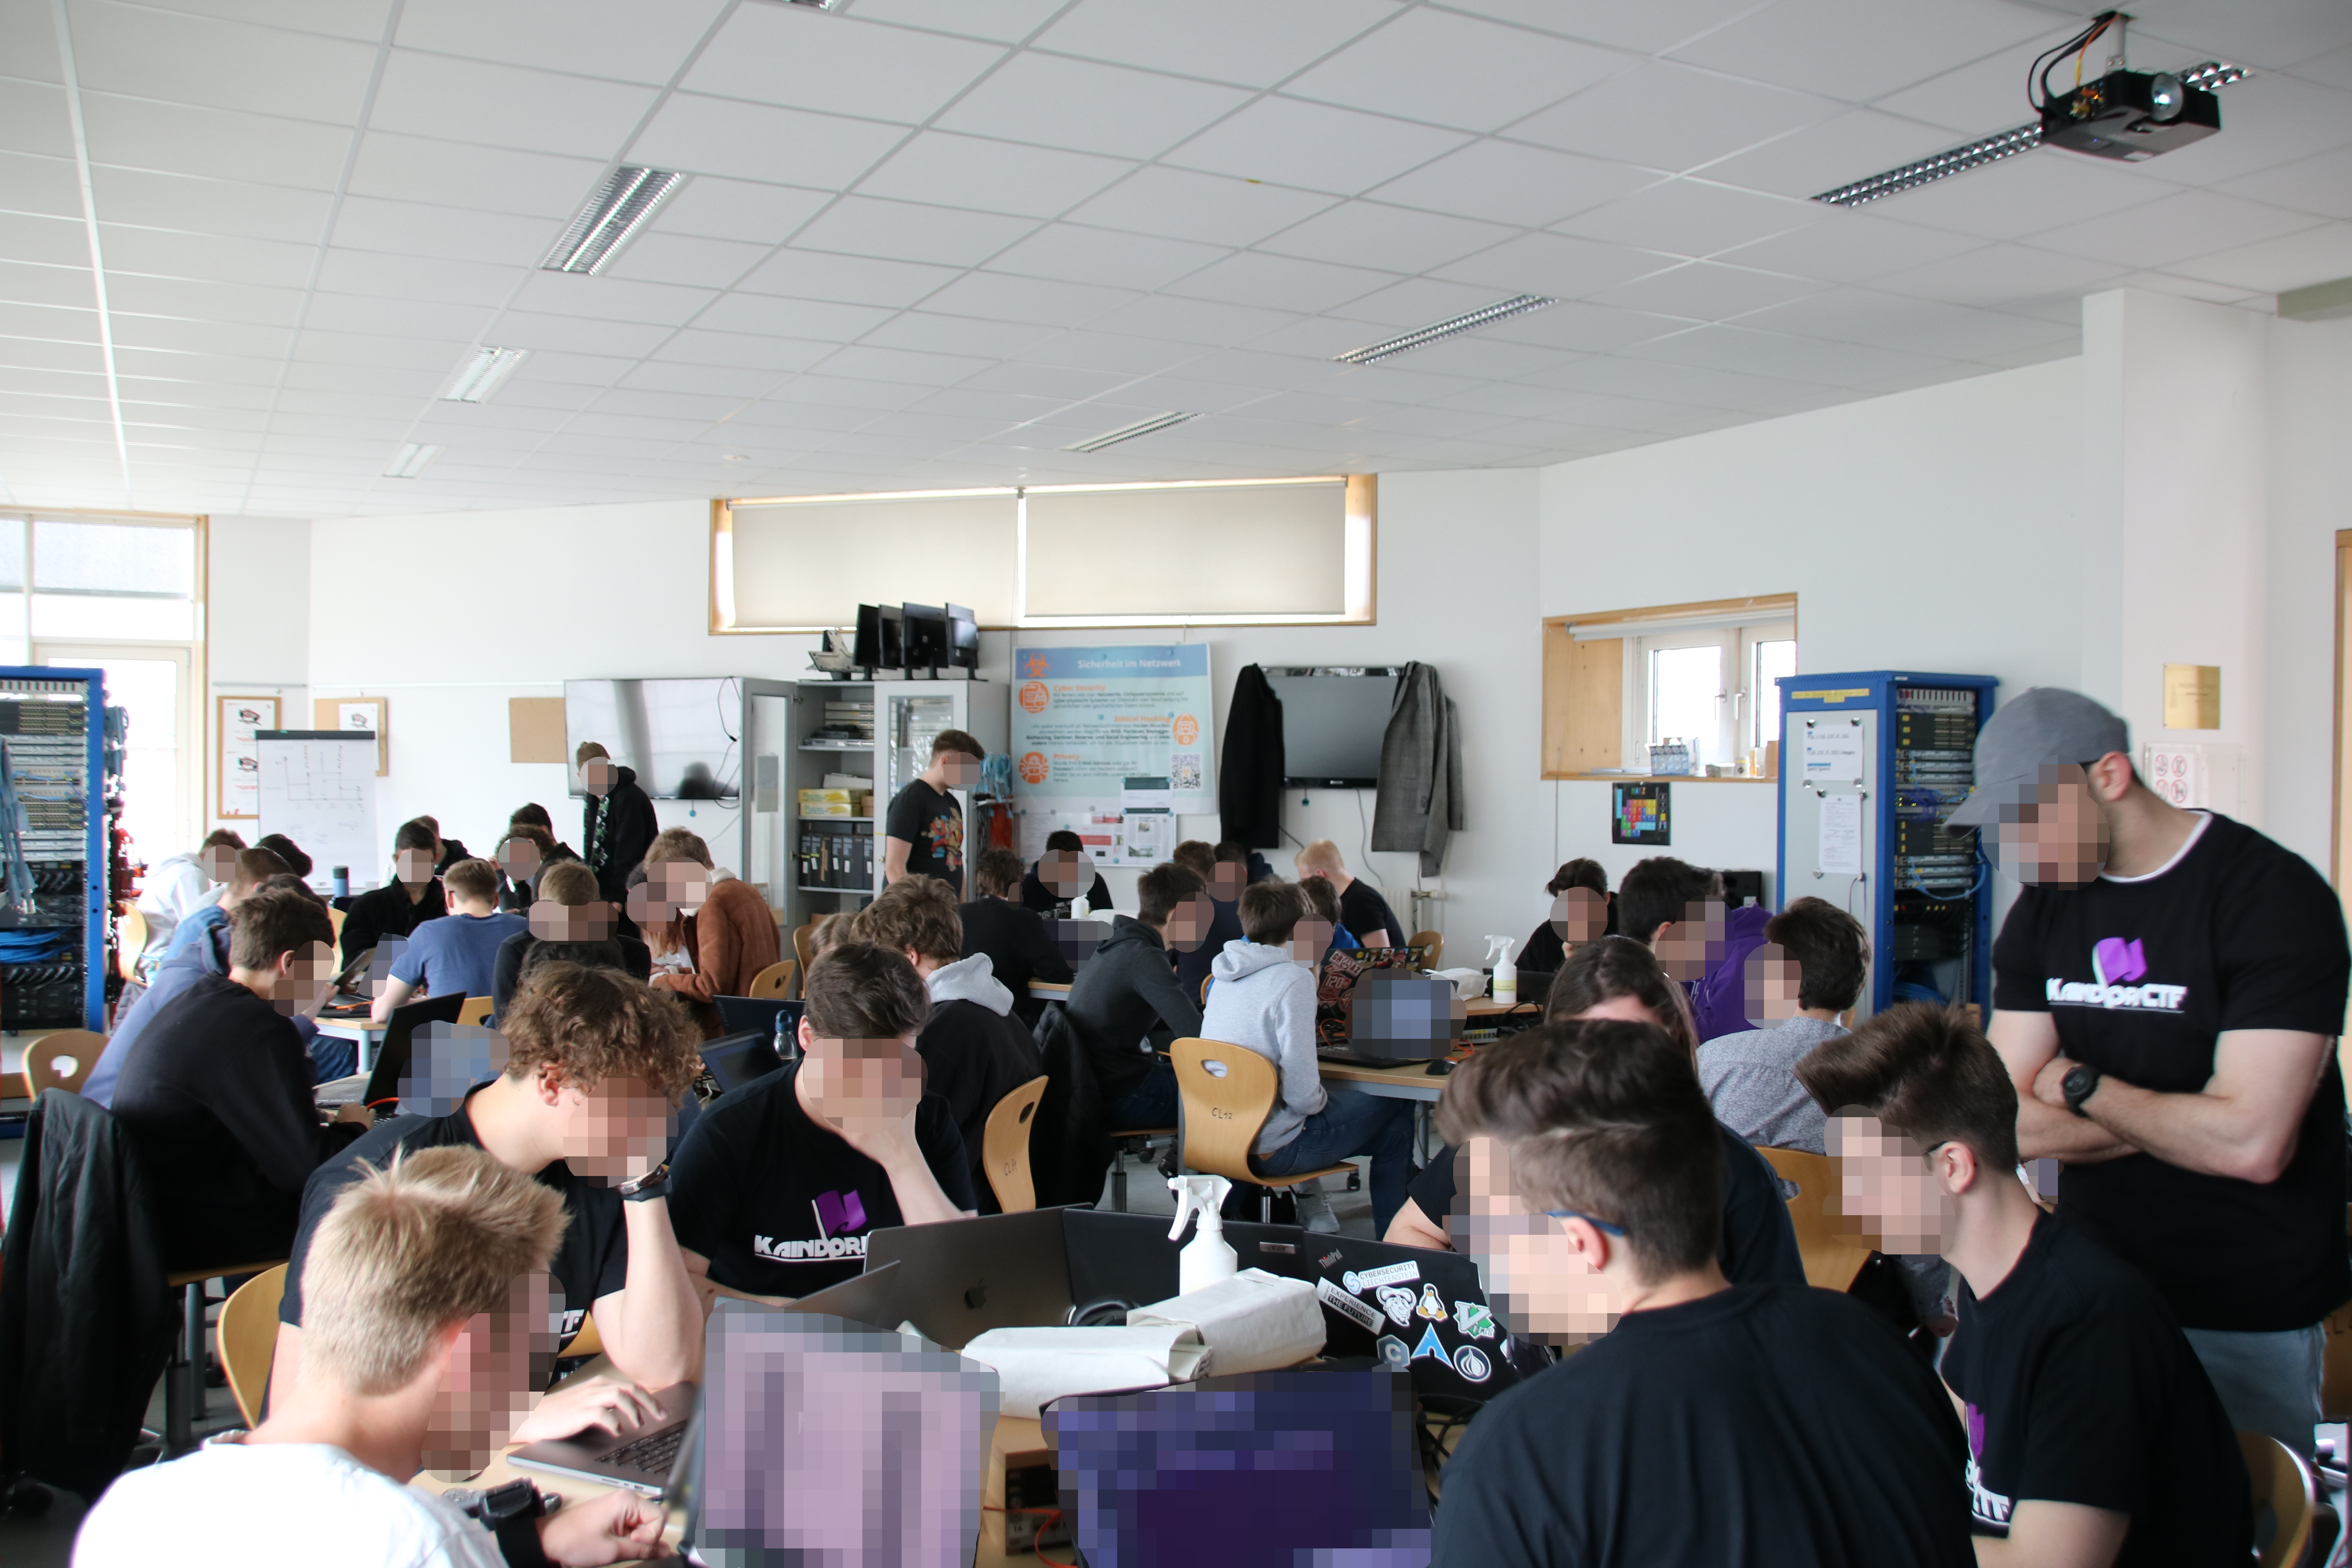
\includegraphics[width=0.45\linewidth]{images/events/kdctf.JPG}
            \end{figure}
        \end{tabular}
    \end{tabular}
\end{frame}

\begin{frame}{Overview}
    What are CTFs?
    \begin{itemize}
        \item {\bf C}apture {\bf t}he {\bf F}lag
        \item Competitions with a focuse on cyber security
        \item Either online (mostly) of offline (typically for finals)
        \item Usually take 24 hours, 36h or even longer
    \end{itemize}
    There are usually the following gamemodes
    \begin{itemize}
        \item Jeopardy (most common)
        \item Attack-Defense
    \end{itemize}
\end{frame}

\begin{frame}{Flag?}
    \huge{LosCTF\{this\_could\_be\_a\_flag\}}
\end{frame}


\section{CTFTime}
\begin{frame}{ctftime.org}
    \centering
    \includegraphics[width=0.8\columnwidth]{images/CTFTimeStartpage.png}
\end{frame}


\section{Jeopardy-CTFs}
\begin{frame}{Challenge Categories}
    Most of the time, challenges fall in one of these Categories
    \begin{itemize}
        \item Reverse engineering
        \item Binary exploitation
        \item Websecurity
        \item Cryprography
        \item Miscellaneous
    \end{itemize}

    Other categories can be
    \begin{itemize}
        \item Web3 (Smart contract security)
        \item Digital forensics 
        \item Programming challenges
        \item Open-source intelligence gathering (OSINT)
    \end{itemize}
\end{frame}

\begin{frame}{How do Jeopardy-CTFs work?}

    \only<1>{
        \centering
        \includegraphics[width=0.95\columnwidth]{images/jeopardy_ctfs/fuzzy_land_1.png}
    }%
    \only<2>{
        \centering
        \includegraphics[width=0.95\columnwidth]{images/jeopardy_ctfs/fuzzy_land_2.png}
    }%
    \only<3>{
        \centering
        \includegraphics[width=0.95\columnwidth]{images/jeopardy_ctfs/fuzzy_land_3.png}
    }%
    \only<4>{
        \centering
        \includegraphics[width=0.95\columnwidth]{images/jeopardy_ctfs/fuzzy_land_4.png}
    }%

\end{frame}


\section{AD-CTFs}
\begin{frame}{Challenge Categories}
    Every team gets a server with vulnerable services \\
    Goals
    \begin{itemize}
        \item Fix the own services
        \item Exploit the other teams
    \end{itemize}

    Typical categories
    \begin{itemize}
        \item Reverse engineering
        \item Binary exploitation
        \item Websecurity
    \end{itemize}
\end{frame}

\begin{frame}{How do AD-CTFs work?}

    \only<1>{
        \centering
        \includegraphics[width=0.95\columnwidth]{images/ad_ctfs/ad_overview_1.png}
    }%
    \only<2>{
        \centering
        \includegraphics[width=0.95\columnwidth]{images/ad_ctfs/ad_overview_2.png}
    }%
    \only<3>{
        \centering
        \includegraphics[width=0.95\columnwidth]{images/ad_ctfs/ad_overview_3.png}
    }%
    \only<4>{
        \centering
        \includegraphics[width=0.95\columnwidth]{images/ad_ctfs/ad_overview_4.png}
    }%
    \only<5>{
        \centering
        \includegraphics[width=0.95\columnwidth]{images/ad_ctfs/ad_overview_5.png}
    }%

\end{frame}


\section{Introduction Challenges}
\begin{frame}{fuzzy.land}
    We prepaired some challenges for you to try out. \\
    \url{https://fuzzy.land} in the section {\bf Intro to CTFs}
    \begin{itemize}
        \item Buffer Overflow 0 (Binary exploitation)
        \item My first reversing challenge (Reverseengineering)
        \item Session Rookie (Websecurity)
        \item My first Contract (Web3, Blockchain)
        \item Superior roman cipher (Cryptographie)
        \item Network Rookie (Websecurity, Forensics)
    \end{itemize}
    We have Linux\-USB Sticks

\end{frame}

\end{document}